\section{Structural Elements\index{Elements!Structural}}

\subsection*{Bernoulli beam elements\index{Elements!Bernoulli}}
These elements allow to compute the displacements and rotations of structures constituted by Bernoulli beams. \akantu defines them for both 2D and 3D problems in the element types \code{\_bernoulli\_beam\_2} and \code{\_bernoulli\_beam\_3}. A schematic depiction of a beam element is shown in Figure~\ref{fig:elements:bernoulli} and some of its properties are listed in Table~\ref{tab:elements:bernoulli}.

\note{Beam elements are of mixed order: the axial displacement is linearly interpolated while transverse displacements and rotations use cubic shape functions.}

\begin{figure}[htb]
  \centering
  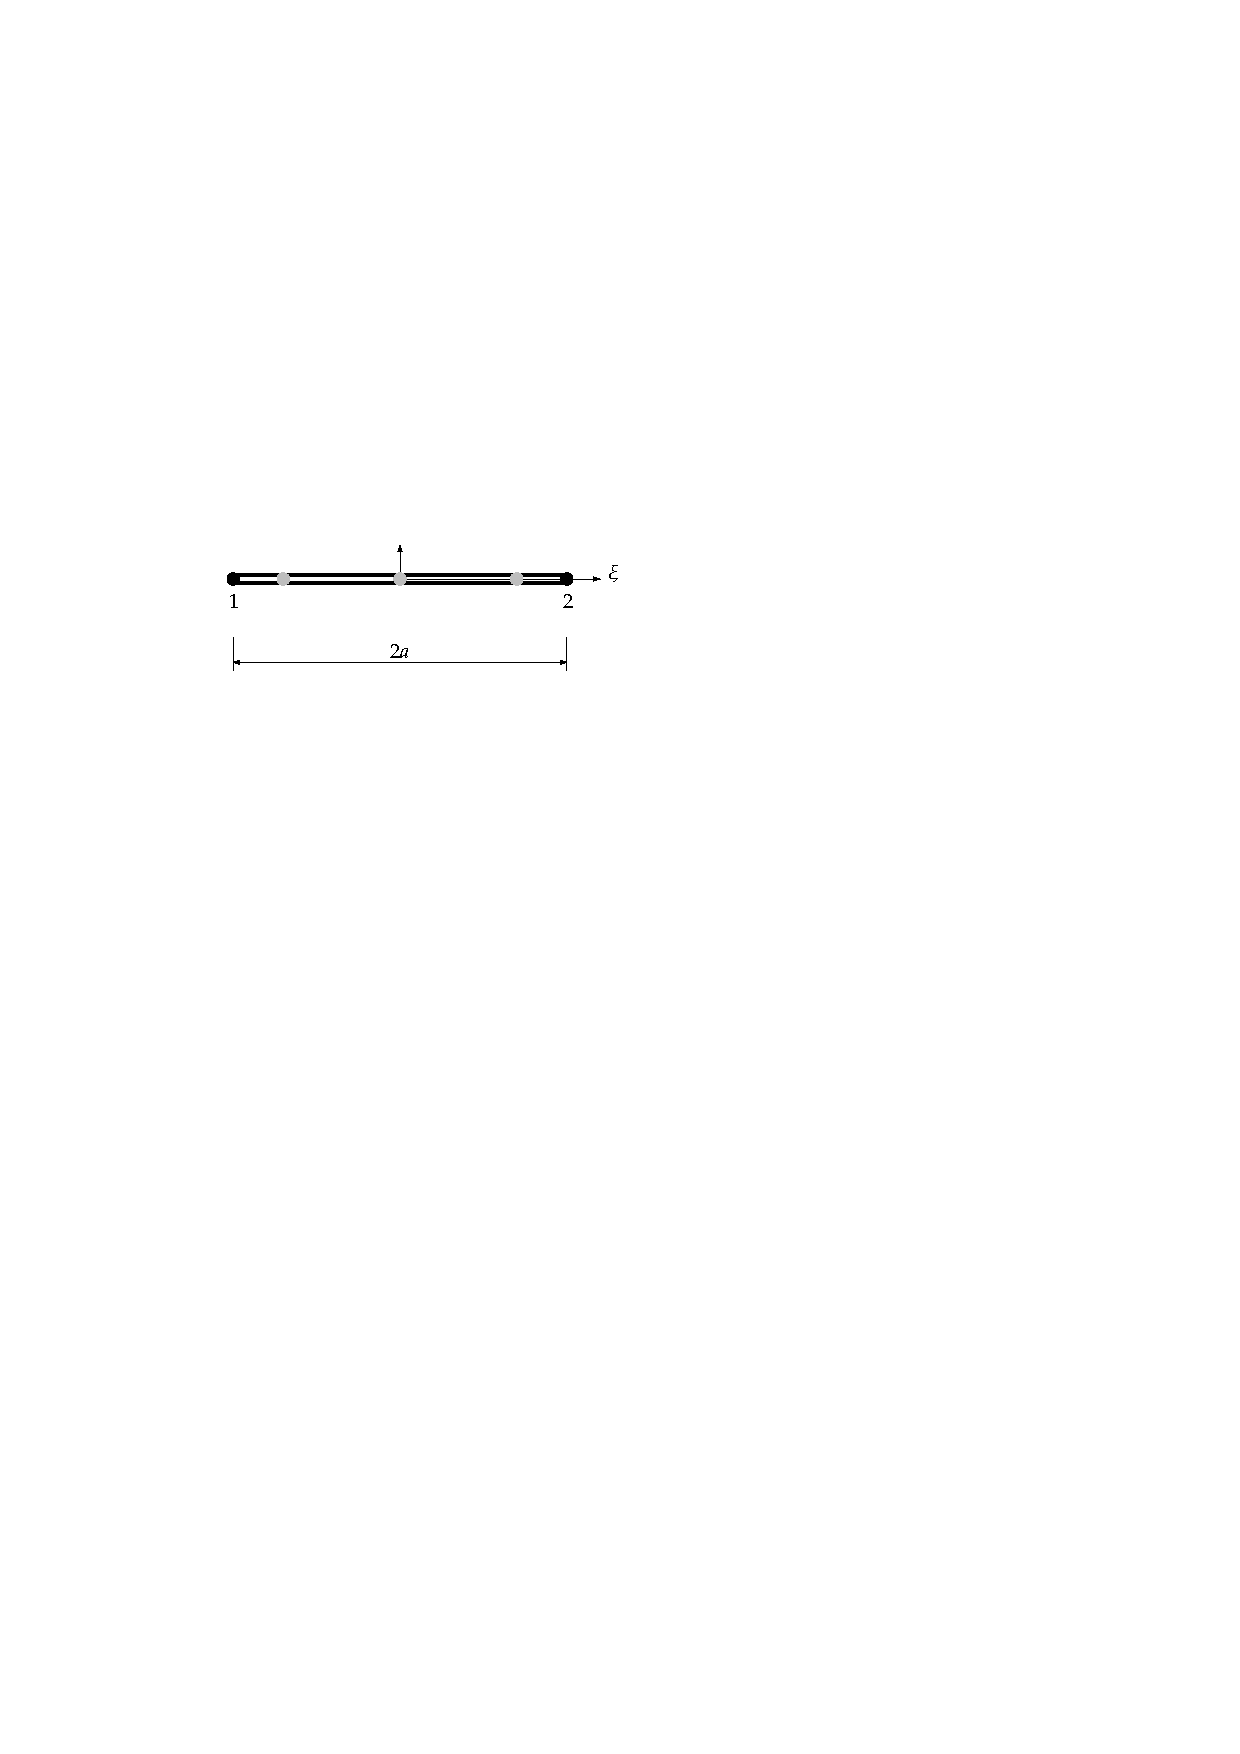
\includegraphics[width=0.3\textwidth]{figures/elements/bernoulli_2}
  \caption{Schematic depiction of a Bernoulli beam element (applied to 2D and 3D) in \akantu. The node numbering as used in \akantu is indicated, and also the quadrature points are highlighted (gray circles).}
  \label{fig:elements:bernoulli}
\end{figure}
\begin{table}[htb]
  \centering
  \begin{tabular}{c|cccc}
    \toprule
    Element type                  & \# Order & \# nodes &\# quad. points & \# d.o.f.\\
    \midrule
    \texttt{\_bernoulli\_beam\_2} &         2&         2&              3&  4\\
    \texttt{\_bernoulli\_beam\_3} &         3&         2&              3&  6\\
    \bottomrule
  \end{tabular}
  \caption{Some basic properties of the beam elements in \akantu}
  \label{tab:elements:bernoulli}
\end{table}
